\documentclass[cnatzke_thesis_proposal.tex]{subfiles}
\begin{document}

\chapter{The GRIFFIN Spectrometer at TRIUMF}

%%%%%%%%%%%%%%%%%%%%
\subsection{TRIUMF Rare Isotope Beam Facility}
%%%%%%%%%%%%%%%%%%%%
\begin{figure}[H]
  \begin{center}
    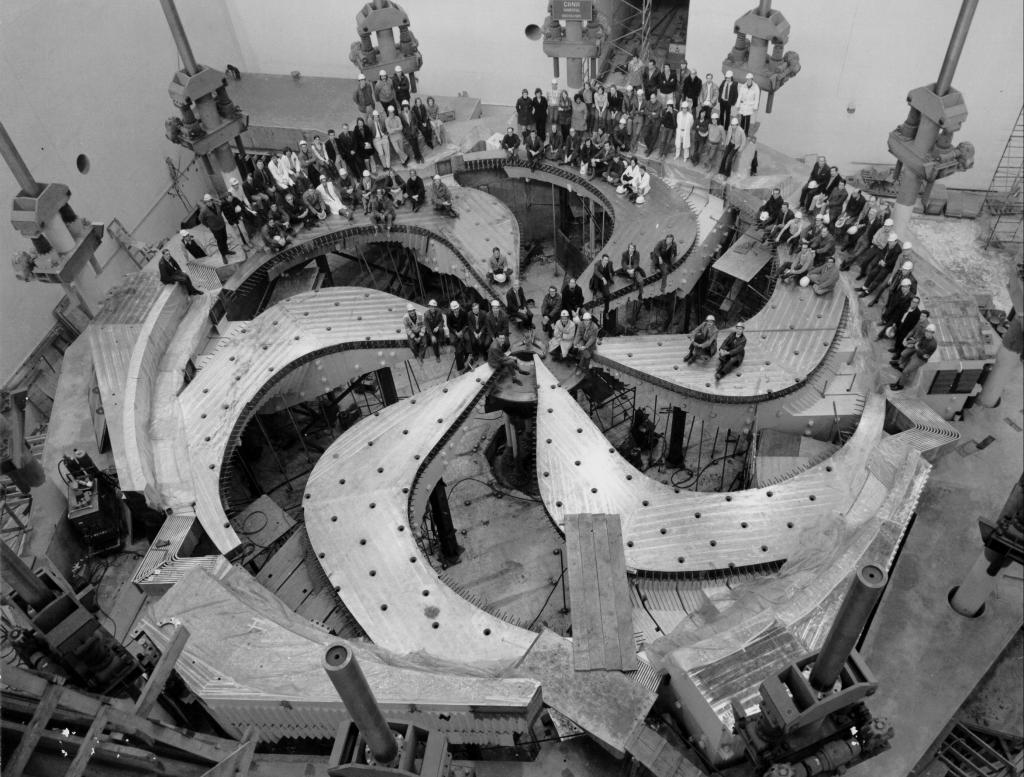
\includegraphics[width=0.95\linewidth]{triumf_cyclotron_construction_1972.jpg}
  \end{center}
  \caption{TRIUMF cyclotron during initial construction (1972) - Figure courtesy of TRIUMF.}
  \label{fig:triumf_cyclotron_1972}
\end{figure}

The proposed experiment will be performed at Canada's national laboratory for nuclear and particle physics, TRIUMF. 
TRIUMF is located in Vancouver, British Columbia, Canada and was established in 1968 by three universities, Simon Fraser University, the University of British Columbia (UBC), and the University of Victoria, as an experimental facility to meet needs the three universities could not individually provide. 
Since then the science program has grown to include nuclear physics, particle physics, molecular and material science, and nuclear medicine while providing research infrastructure and tools too large or complex for a single university to build, operate, or maintain. 
TRIUMF houses the world's largest cyclotron \cite{dilling_isac_2014} capable of accelerating protons up to 520 MeV before they are delivered to the experimental halls, via one of four beam lines, for direct use or to create secondary radioactive isotope beams of pions, muons, or radioactive isotopes. 
This work uses the GRIFFIN spectrometer housed in the ISAC-I experimental hall located on the TRIUMF-ISAC-I experimental hall. 

%%%%%%%%%%%%%%%%%%%%
\subsection{The GRIFFIN Spectrometer}
%%%%%%%%%%%%%%%%%%%%

%\begin{center}
%\begin{figure}[H]
%  \begin{center}
%    \includegraphics[scale=.18]{isac_i_facility.png}
%  \end{center}
%  \caption{Schematic view of the TRIUMF-ISAC facility \cite{Dilling2014}, including the target ion-source, the high resolution mass separator, and various detection stations.}
%  \label{fig:ISAC_HALL}
%\end{figure}
%\end{center}

Large scale detector arrays for $\gamma$-ray measurements provide a powerful and robust tool for studying unstable nuclei through radioactive decay and nuclear spectroscopy at radioactive ion beam facilities \cite{garnsworthy_griffin_2019}. 
The Gamma-Ray Infrastructure For Fundamental Investigations of Nuclei (GRIFFIN) is a Compton-suppressed, high-efficiency $\gamma$-ray spectrometer composed of sixteen large-volume clover-type High Purity Germanium (HPGe) detectors located in the ISAC-I experimental hall at TRIUMF. 
The detectors are arranged to cover sixteen of the eighteen faces of a rhombicuboctahedron with the front faces of the detectors able to be set 110 or 145 mm from the beam implantation location at the centre of the array. 
One of the vacant faces is used for the incoming low-energy RIB from ISAC-I and the other, opposite face is used for the tape collection system that removes long-lived activity from the implantation chamber at the end of a measurement cycle \cite{garnsworthy_griffin_2019}. Each clover contains four large-volume HPGe crystals aligned to the tape system where the radioactive beam is implanted and decays. 
The western hemisphere of GRIFFIN is shown in Figure \ref{fig:griffin_westhemi} where the upstream beam line can be seen on the rightmost edge of the image. 

\begin{center}
  \begin{figure}[H]
    \begin{center}
      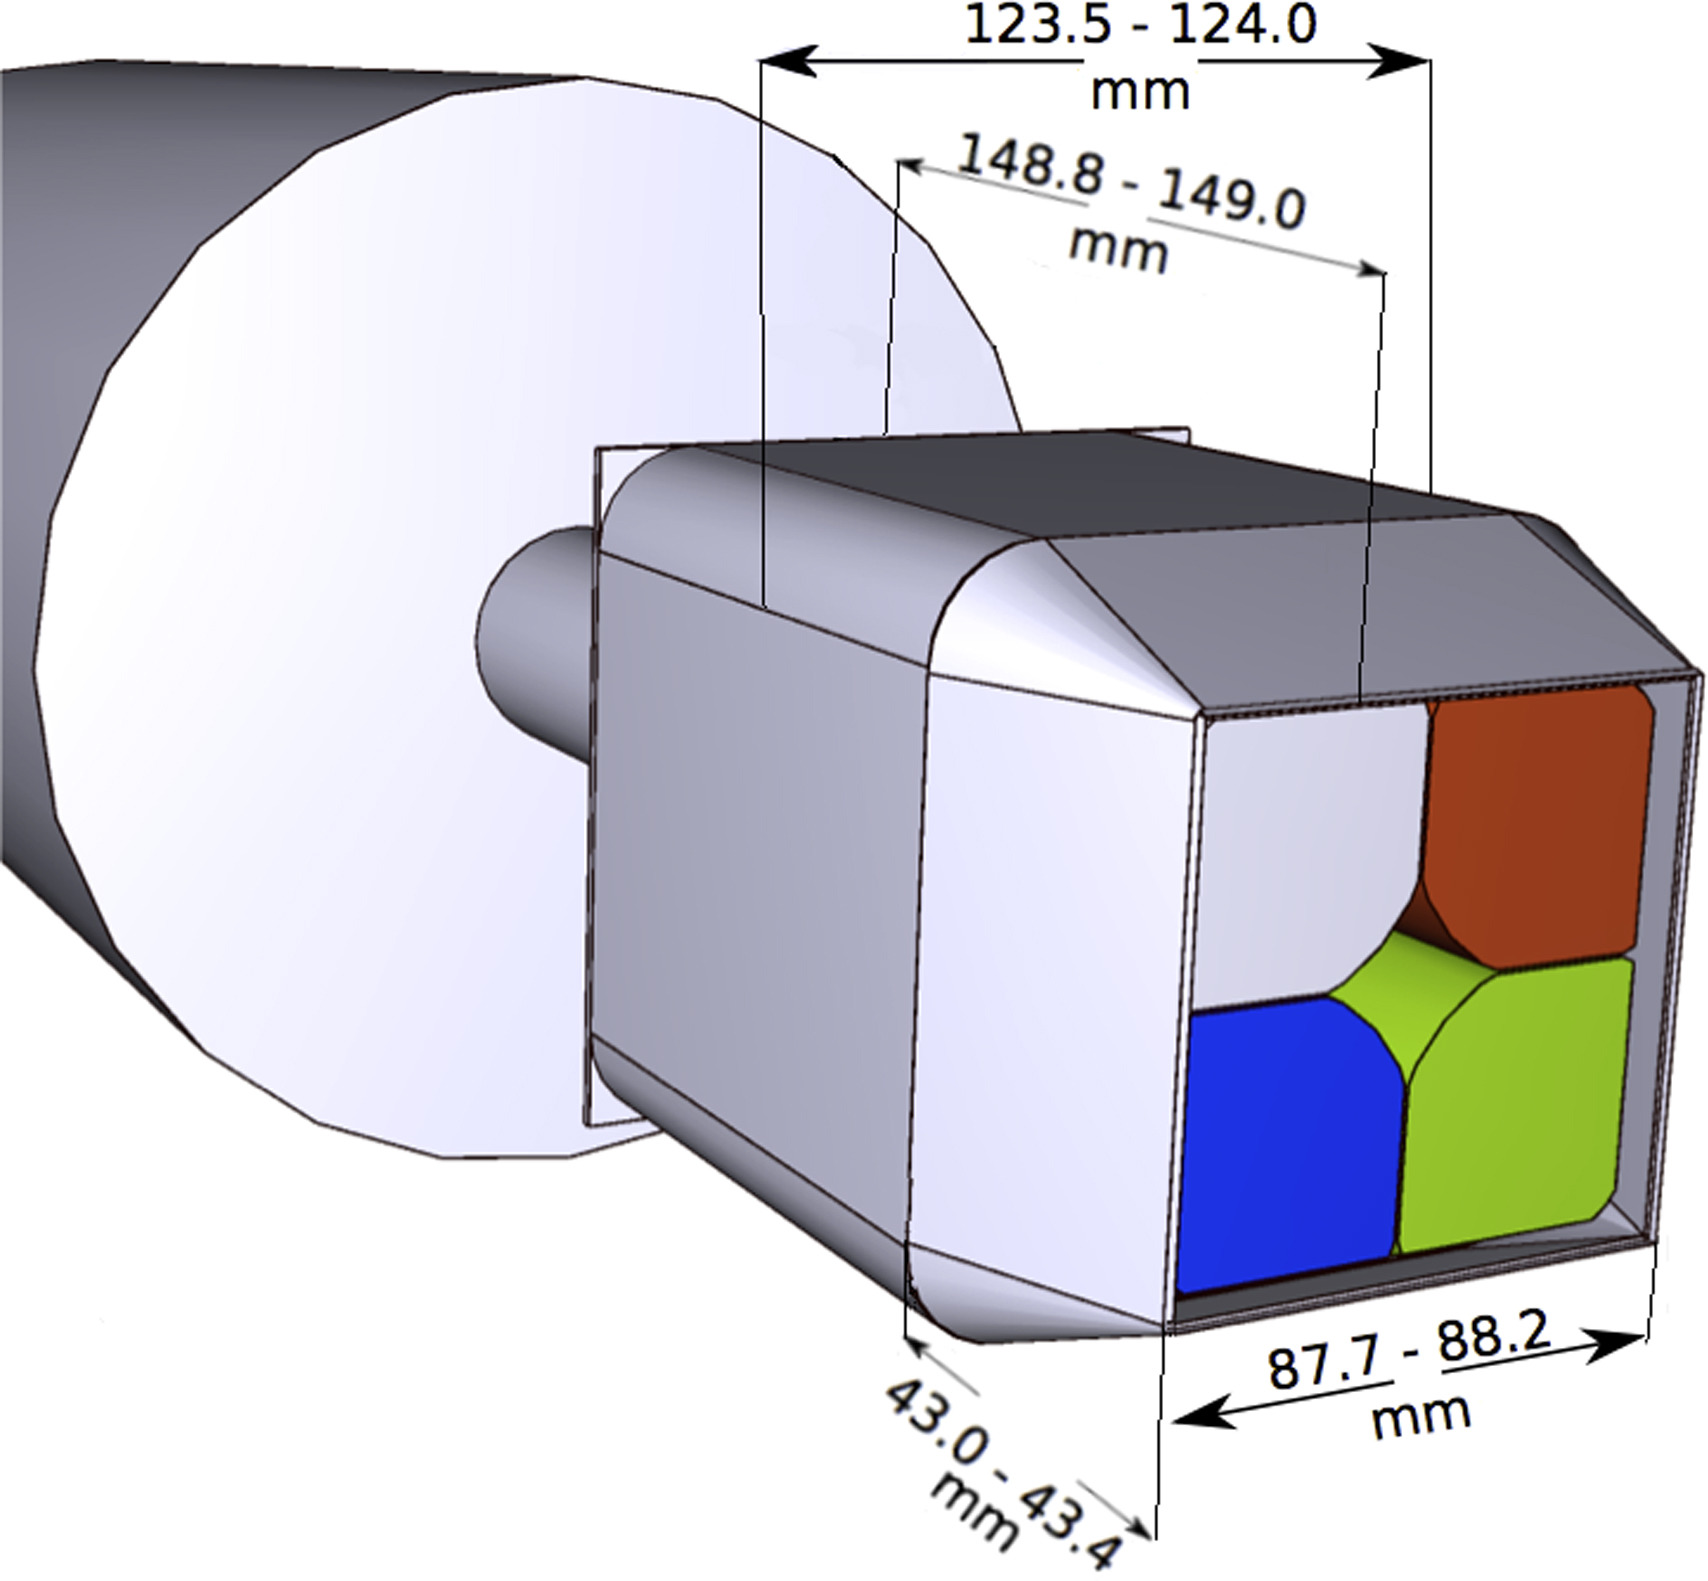
\includegraphics[width=0.95\textwidth]{griffin_clover_schematic.jpg}
    \end{center}
    \caption{Rendering of a GRIFFIN HPGe clover with the exterior dimensional tolerances of the aluminum crystal housing indicated. Figure from Ref.~\cite{rizwan_characteristics_2016}.}
    \label{fig:griffin_clover_schematic}
  \end{figure}
\end{center}

\begin{center}
  \begin{figure}[H]
    \begin{center}
      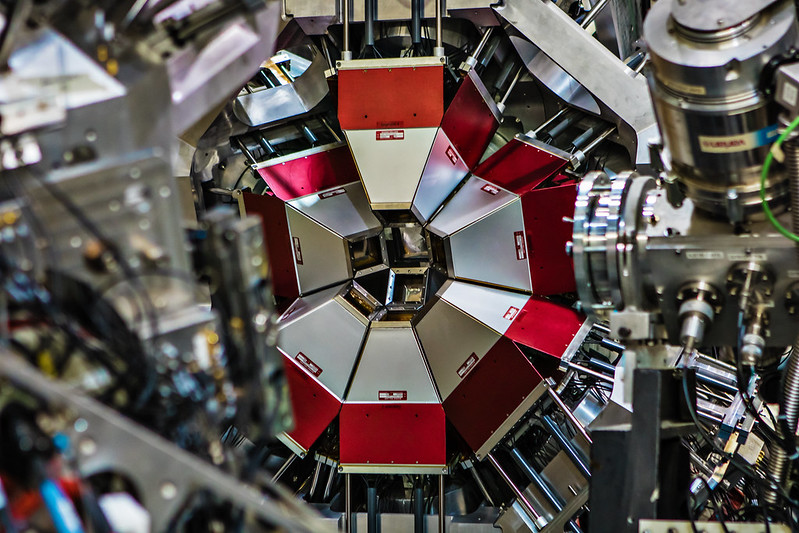
\includegraphics[width=0.95\textwidth]{griffin_westhemi.jpg}
    \end{center}
    \caption{Western hemisphere of GRIFFIN in optimized-peak-to-total mode taken during TRIUMF photowalk 2018. Image by Matthias Le Dall.}
    \label{fig:griffin_westhemi}
  \end{figure}
\end{center}

Each GRIFFIN clover is surrounded by a set of bismuth germanate (BGO) active Compton suppression shields used to detect $\gamma$-rays that have scattered out of a HPGe crystal and 511 keV $\gamma$-rays created via pair production. 
The BGO shields are made of a high-density, large atomic number ($Z$ = 83 for Bi) scintillator coupled to a photomultiplier tube (PMT) to create a detector ideally suited to measure escaping $\gamma$-rays due to its high $\gamma$-ray interaction cross-section. 

The GRIFFIN spectrometer has two distinct operating configurations based on the relative position of the BGO suppression shields and HPGe clover faces to the centre of the array. 
The first of which named "high-efficiency mode" is when the clovers are 110 mm radially distant from the centre of the array and the front BGO shields are pulled back, shown in the top panel of Figure~\ref{fig:griffin_modes}, to facilitate a large solid angle coverage and greater absolute detection efficiency. 
The second mode, called "optimized peak-to-total" mode shown in the bottom panel of Figure~\ref{fig:griffin_modes}, is when the HPGe clovers are 145 mm from the centre of the array and the front shield plates of the BGO suppressors are rolled forward to form a complete suppression shield around each HPGe clover. 

\begin{center}
  \begin{figure}[H]
    \begin{center}
      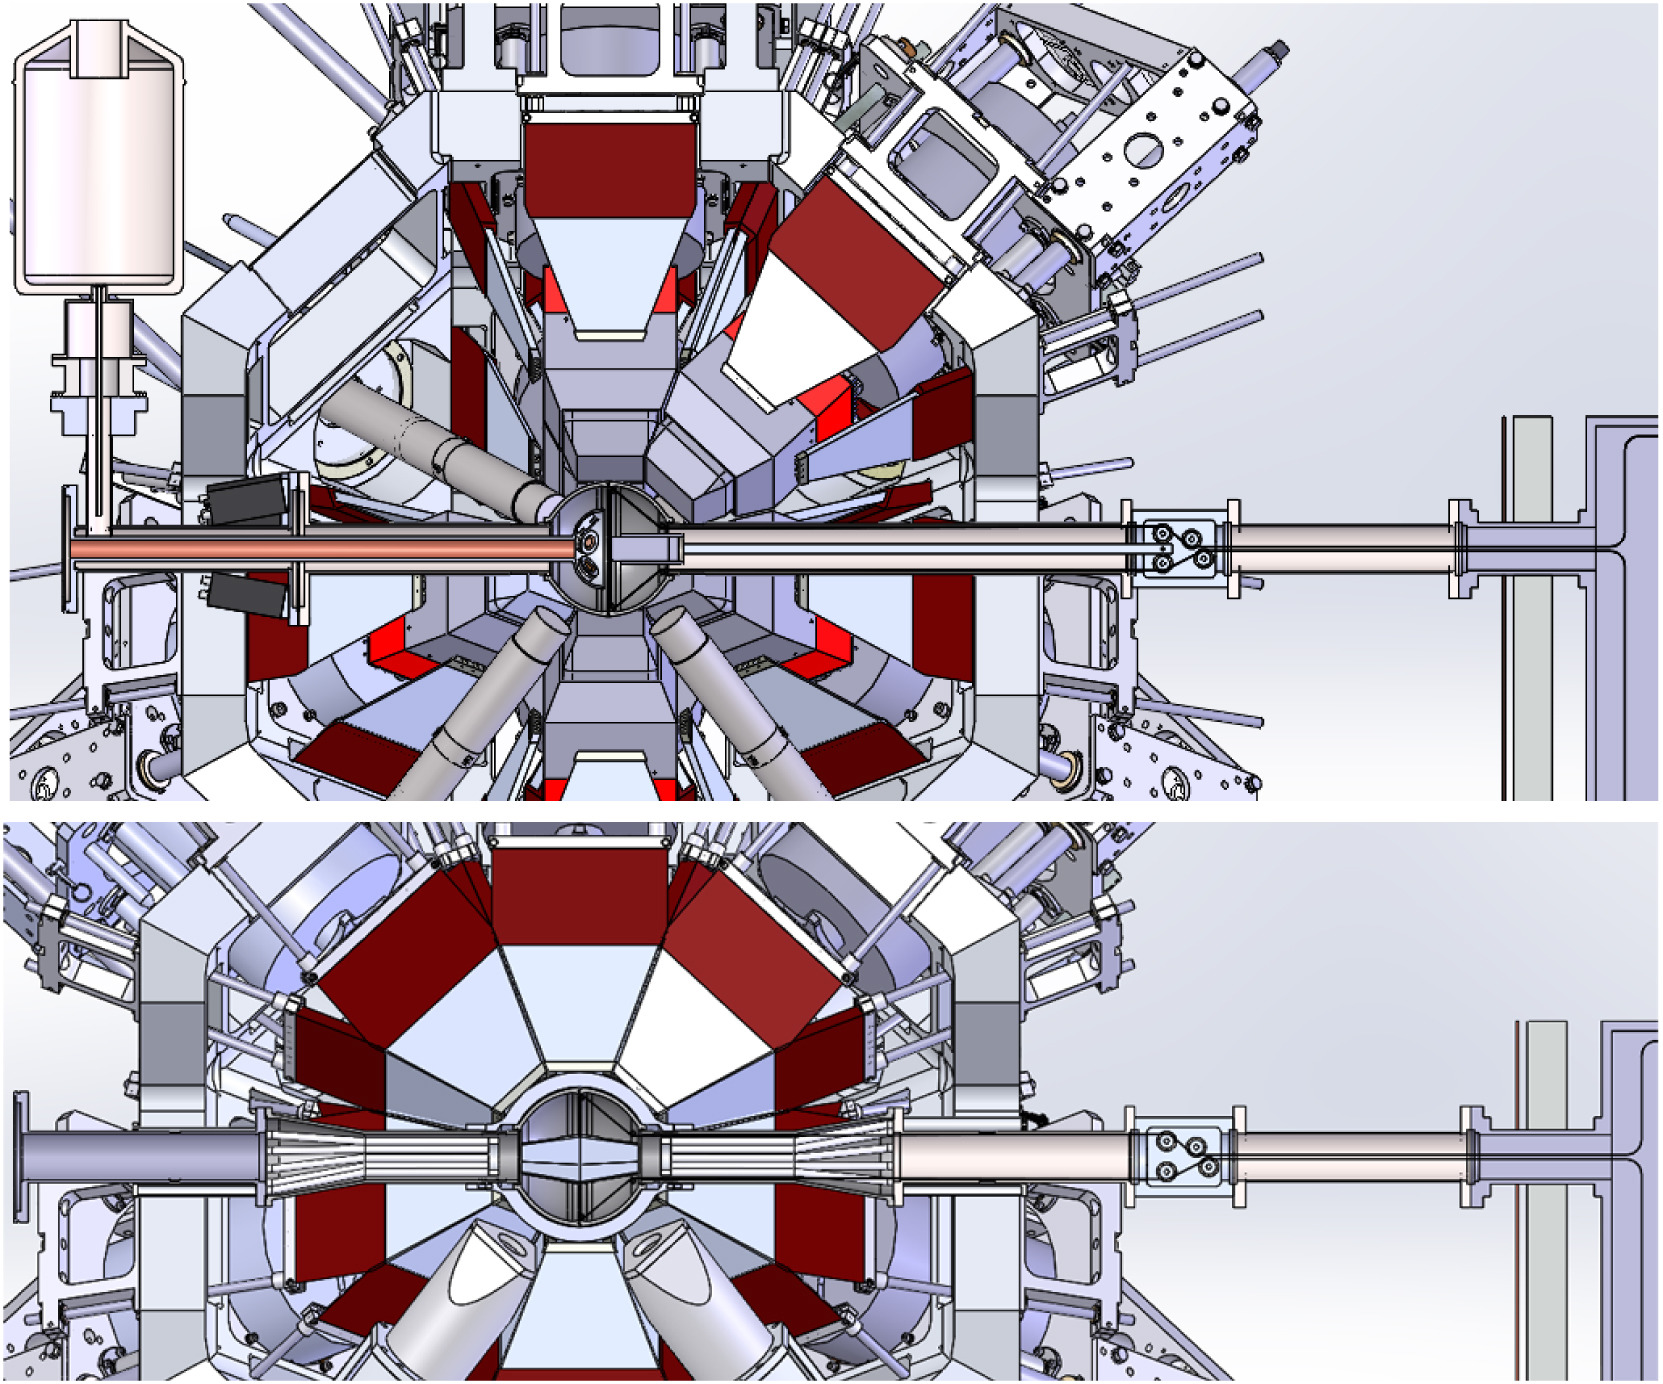
\includegraphics[width=0.95\textwidth]{griffin_modes.jpg}
    \end{center}
    \caption{Two possible configurations of the GRIFFIN spectrometer. The beam is delivered from the left. The Pb wall shielding the tape box can be seen on the right. Upper panel showing PACES in the upstream (left) half of the chamber and the fast scintillator in the downstream (right) chamber. In the ‘High-efficiency’ mode, the HPGe detectors are at 11 cm and the LaBr(Ce) detectors at 12.5 cm from the implantation point on the tape. Lower panel with SCEPTAR in the upstream and downstream chambers. In the ‘Optimized peak-to-total’ mode, the HPGe and LaBr(Ce) detectors are retracted to 14.5 cm and 13.5 cm, respectively, in order that they can be fully Compton and background suppressed with BGO shields. The 20 mm Delrin absorber is also installed in the lower panel. Figure taken from Ref. \cite{garnsworthy_griffin_2019}.}
    \label{fig:griffin_modes}
  \end{figure}
\end{center}


% ------------------------------------
\end{document}
